\iffalse
\bibliography{ref.bib}
\fi

\section{Results}
We perform a variety of experiments across different tasks and neural network architectures in natural language processing as well as image classification. We report our experimental findings on language tasks in section~\ref{sec:NLP}, and image classification
in section~\ref{sec:image_class}. We illustrate that CBS schedules can alleviate sub-optimal initialization in section~\ref{sec:bad_init}. We follow the baseline training method for each task (for details please see Appendix~\ref{sec:training_outline}). 
Alongside testing/validation performance, we also report the number of training iterations (lower values are preferred).

\subsection{Language Results}\label{sec:NLP}

Language modeling is a challenging problem due to the complex and long-range interactions between distant words~\cite{merity2016pointer}.
One hope is that large/deep models might be able to 
capture these complex interactions, but large models easily overfit on these tasks and exhibit large gaps between training set and testing set performance. 
CBS schedules effectively help us avoid overfitting, and in addition snapshot ensembling enables even greater performance.

\begin{table}[!htbp]
\caption{\footnotesize Testing perplexity and number of parameter updates of L1 and L2 models on Penn 
Tree Bank (PTB) and WikiText~2 (WT2) datasets. The best perplexity and lowest number of 
updates are \textbf{bolded}. }
\label{tab:lm-results}
\centering
\begin{tabular}{lcc|cc|cc|cc} \toprule
  &\multicolumn{2}{c}{L1 on PTB}       &\multicolumn{2}{c}{L1 on WT2}    &\multicolumn{2}{c}{L2 on PTB} &\multicolumn{2}{c}{L2 on WT2}\\              
\midrule
Schedule    & {Per.}    & {\# Iters}    & {Per.}    & {\# Iters}    & {Per.}     & {\# Iters}   & {Per.}    & {\# Iters}      \\
\midrule
\Gc	BL\footnotemark	&	83.13	&	52k	&	96.41	&	116k	&	79.34	&	73k	&	99.69	&	164k	\\
\midrule
\Ga	CBS-10	&	80.49	&	49k	&	94.93	&	111k	&	79.37	&	83k	&	95.43	&	187k	\\
\Gc	CBS-5	&	80.78	&	49k	&	\textbf{94.31}	&	111k	&	78.61	&	73k	&	94.32	&	164k	\\
\Ga	CBS-1	&	81.56	&	49k	&	94.52	&	111k	&	77.56	&	69k	&	\textbf{91.78}	&	156k	\\
\midrule
\Gc	CBS-10-A	&	\textbf{80.28}	&	35k	&	95.91	&	79k	&	81.47	&	65k	&	95.28	&	146k	\\
\Ga	CBS-5-A	&	82.03	&	35k	&	95.23	&	79k	&	79.48	&	53k	&	93.63	&	118k	\\
\Gc	CBS-1-A	&	84.41	&	35k	&	95.66	&	79k	&	81.32	&	49k	&	93.19	&	111k	\\
\midrule
\Ga	CBS-10-T	&	80.49	&	49k	&	94.93	&	111k	&	79.42	&	83k	&	94.39	&	187k	\\
\Gc	CBS-5-T	&	80.94	&	53k	&	94.9	&	120k	&	78.95	&	63k	&	94.68	&	142k	\\
\Ga	CBS-1-T	&	81.82	&	46k	&	95.38	&	104k	&	\textbf{77.39}	&	65k	&	93.78	&	147k	\\
\bottomrule 
\end{tabular}
\end{table}

We evaluate a large variety of CBS schedules to positive results as shown in~\tref{tab:lm-results}. 
Results are measured in perplexity, a standard figure of merit for evaluating the quality of language models by measuring its prediction of the empirical distribution of words (lower perplexity value is better). 
As we can see, the best performing CBS schedules result in significant improvements in
perplexity (up to 7.91) over the baseline schedules and also offer reductions in the number of SGD training iterations (up to $33\%$). For example, CBS schedules achieve improvement of 7.91 perplexity improvement on WikiText~2 via CBS-1-T and reduce the SGD iterations from 164k to 111k via the CBS-1-A schedule.
Notice that almost all CBS schedules outperform the baseline schedule.
\begin{figure}[!htbp]
  \centering
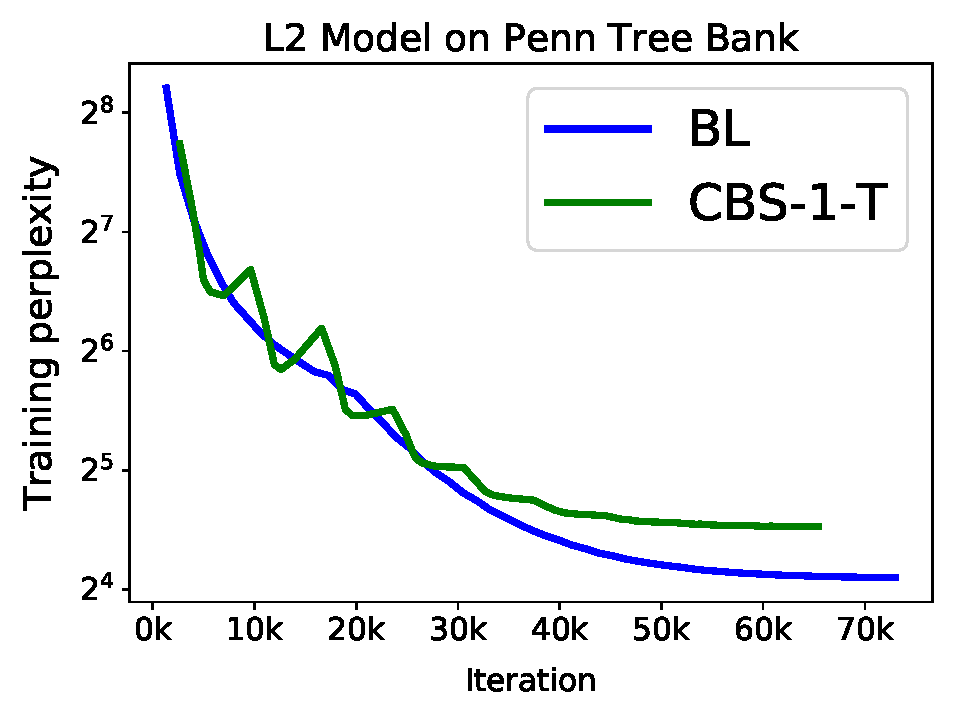
\includegraphics[width=.4\textwidth]{fig/train_l2_ptb.pdf}
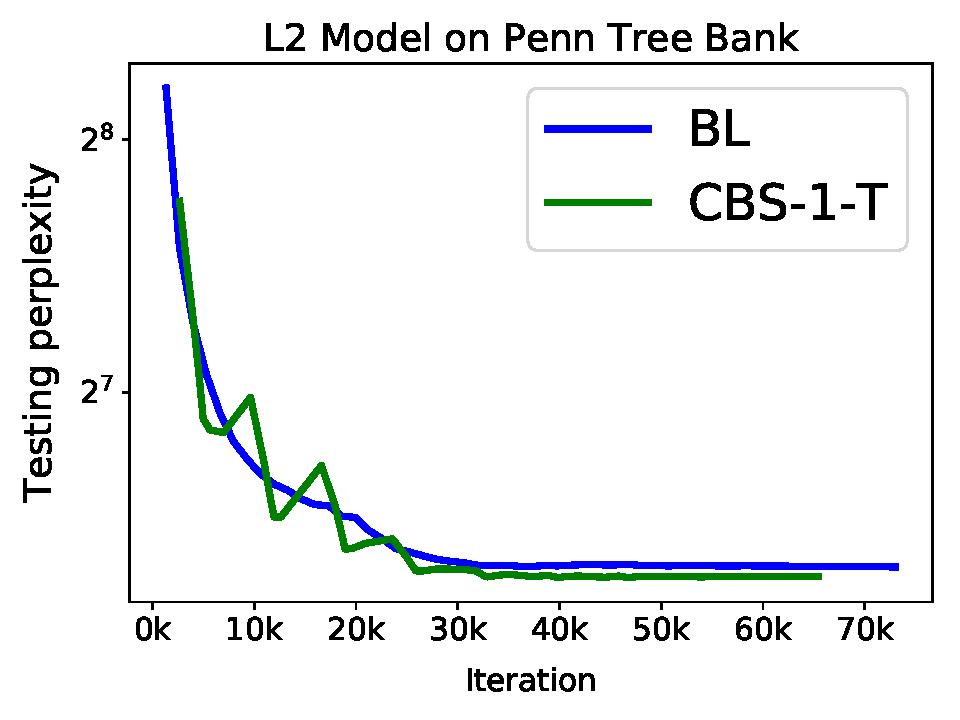
\includegraphics[width=.4\textwidth]{fig/test_l2_ptb.pdf}
  \caption{\footnotesize Training (left) and testing (right) perplexity as a function of iterations for the L2 model on PTB.}
  \label{fig:l2_ptb}
\end{figure}

\fref{fig:l2_ptb} shows the training and testing perplexity of the L2 model on PTB and WikiTest~2 as trained via the baseline schedule 
along with our best CBS schedule (from \tref{tab:lm-results}). Notice the cyclical spikes in training and testing perplexity. The peaks occur during  decreases in batch size, i.e., increases in noise scale, which could help to escape sub-optimal local minima, and the troughs occur during increases in batch size, i.e., decreases with noise scale.

In order to support our claim that CBS schedules are especially useful for counteracting overfitting, we conducted additional language modeling experiments on models L1', L2' with PTB and WT2 which use significantly lower dropout (0.2 and 0.3) than the original L1, L2 models (0.5 and 0.65). Because these models heavily overfit the training data, we report both the final testing perplexity as well as the best testing perplexity achieve during training. 
As seen in \tref{tab:lm-results-overfit} (in Appendix~\ref{sxn:app:additional results}), with L2' CBS yields improvements of a staggering 60.3 on final testing perplexity and 36.2 on best testing perplexity. CBS yields smaller improvements on L1' of 26.0 and 25.3, which are still much larger than the improvement achieved by CBS on L1 and L2. 


As mentioned above the goal of every cycle is to get an approximate MAP point. A very interesting idea
proposed in~\citep{huang2017snapshot} is to ensemble these MAP points by saving snapshots of the model
at the end of every cycle. We follow that strategy with the only difference that we use a batch size cycle
instead of cyclical learning rate proposed in~\citep{huang2017snapshot} due to higher parallelization opportunities for the former.
We perform experiments on snapshot ensembling with the L2 model with the respective best performing CBS schedules on PTB and WikiText~2 (CBS-1-T and CBS-1), as well as the fixed batch size baseline.
The CBS ensembles on PTB and WikiText~2 result in test set perplexity of 76.14 and 88.47, outperforming baseline ensembles on both datasets (76.52, 89.99 respectively) and CBS single models (77.39, 91.78 respectively).


To further explore the properties of cyclical batch size schedules, we also evaluate these schedules on natural language inference tasks, as shown in~\tref{tab:nli-results}. In our experiments, CBS schedules do not yield large performance improvements on models like E1 which exhibit smaller disparities between training and testing performance.
This is in line with our limitation in that CBS is more effective for models which tend to overfit. On the other hand, we see a large reduction in training 
iterations by up to 62\% which is due to higher effective batch size used in CBS than baseline.


\footnotetext{\citep{zaremba2014recurrent} reports testing perplexity of 82.7 and 78.4 
for L1 and L2 respectively on PTB, which we could not reproduce. The best perplexity and lowest number of updates are \textbf{bolded}.}

\begin{wraptable}{r}{7cm}
\caption{\footnotesize Validation accuracy and number of parameter updates of E1 on MultiNLI and SNLI 
datasets. The best accuracy and lowest number of updates are \textbf{bolded}. }
\label{tab:nli-results}
\centering
\begin{tabular}{lcc|cc} \toprule
  &\multicolumn{2}{c}{MultiNLI}       &\multicolumn{2}{c}{SNLI}    \\              
\midrule
Strategy    & {Acc.}    & {\# Iters}    & {Acc.}    & {\# Iters}    \\
\midrule
\Gc	BL	    &	72.87	&	123k	&	\textbf{86.86}	&	172k	\\
\Ga	CBS-1	&	\textbf{73.17}	&	64k	&	86.73   &   90k   \\
\Gc	CBS-2	&	73.07	&	71k	&	86.56   &   99k	\\
\Ga CBS-1-A &   72.23   & \textbf{48k}     & 86.26     & \textbf{67k}     \\
\Gc CBS-2-A &   72.04   & 57k     & 85.83     & 80k     \\
\bottomrule 
\end{tabular}
\end{wraptable}


\subsection{Image Classification Results}\label{sec:image_class}
We also test our CBS schedules on Cifar-10 and ImageNet. Table.~\ref{tab:cbs_cifar10} reports the testing accuracy and the number of training iterations for different models on Cifar-10. We see that the CBS schedules match baseline performance, but the number of training iterations used in CBS schedules is up to $2\times$ fewer. 

As seen in \fref{fig:wresnet_cifar10}, the training curves of CBS schedules also 
exhibit the aforementioned cyclical spikes both in training loss and testing 
accuracy. Similarly in the previously discussed language experiments, these spikes correspond to cycles in the CBS schedules and can 
be thought of as re-initializations of the neural network weights. We observe that CBS achieves similar performance to the baseline. 


\fref{fig:cbs_imagenet} shows the results of ResNet50 on ImageNet. The baseline trains in  $450k$ 
iterations and reaches $76.134\%$ validation accuracy. With CBS, the final validation accuracy is 
$76.336\%$, trained in $262k$ parameter updates.
CBS outperforms the baseline on both training loss and validation accuracy. 

We offer further support for the hypothesis that CBS schedules are more effective for overfitting neural networks with experiments on model C4, which achieves 94.35\% training 
accuracy 
and 55.55\% testing accuracy on Cifar-10. With CBS-15, we see 90.71\% training 
accuracy 
and 56.44\% testing accuracy, which is a larger improvement than that offered by CBS on convolutional models on Cifar-10.

We also explore combining CBS with the recent adversarial regularization proposed by~\cite{yao2018large}.
Combining CBS-15 on C2 with this strategy improves accuracy to $94.82\%$. This outperforms other schedules shown in  Table~\ref{tab:cbs_cifar10}.
Applying snapshot ensembling on C3 trained with CBS-15-2 leads to improved accuracy of $93.56\%$ as compared to $92.58\%$.
After ensembling ResNet50 on Imagenet with snapshots from the last two cycles, the performance increases to 76.401\% from 75.336\%.

\begin{table}[!htbp]
\caption{\footnotesize Accuracy and number of parameter updates of different models on Cifar-10. The best accuracy and lowest number of iterations are \textbf{bolded}.}
\label{tab:cbs_cifar10}
\centering
\begin{tabular}{lcc|lcc|lcc} \toprule
\multicolumn{3}{c}{AlexNet-like (C1)}  &\multicolumn{3}{c}{WResNet (C2)}  &\multicolumn{3}{c}{ResNet18 (C3)} \\              
\midrule
    {Strategy}                  & {Acc.} & {\# Iters}               &{Strategy}           & {Acc.} & {\# Iters}        &{Strategy}           & {Acc.} & {\# Iters}                     \\
    \midrule
\Gc  Baseline             &86.94            & 35k            & Baseline     &94.53   & 78k                   & Baseline      & \textbf{92.71}  & 63k          \\
\Ga  CBS-10-3          &86.83            & 20k               & CBS-15       &94.46   & 40k                   & CBS-10 & 92.47 & \textbf{32k}         \\
\Gc  CBS-15-2          &86.87            & 26k               & CBS-10-3     &\textbf{94.56}   & 45k          & CBS-5-3  & 92.45 & 37k        \\
\Ga  CBS-5-3           &\textbf{87.03}   & 20k      & CBS-5-3      &94.44   & 45k                   & CBS-15-2 & 92.58 & 48k         \\
\Gc  CBS-5-3-A         &86.75            & \textbf{15k}               & CBS-5-3-A    &94.34   & \textbf{33k}          & CBS-15-2-A & 92.27 & 39k             \\
     \bottomrule 
\end{tabular}
\end{table}



\begin{figure}[!htbp]
  \centering
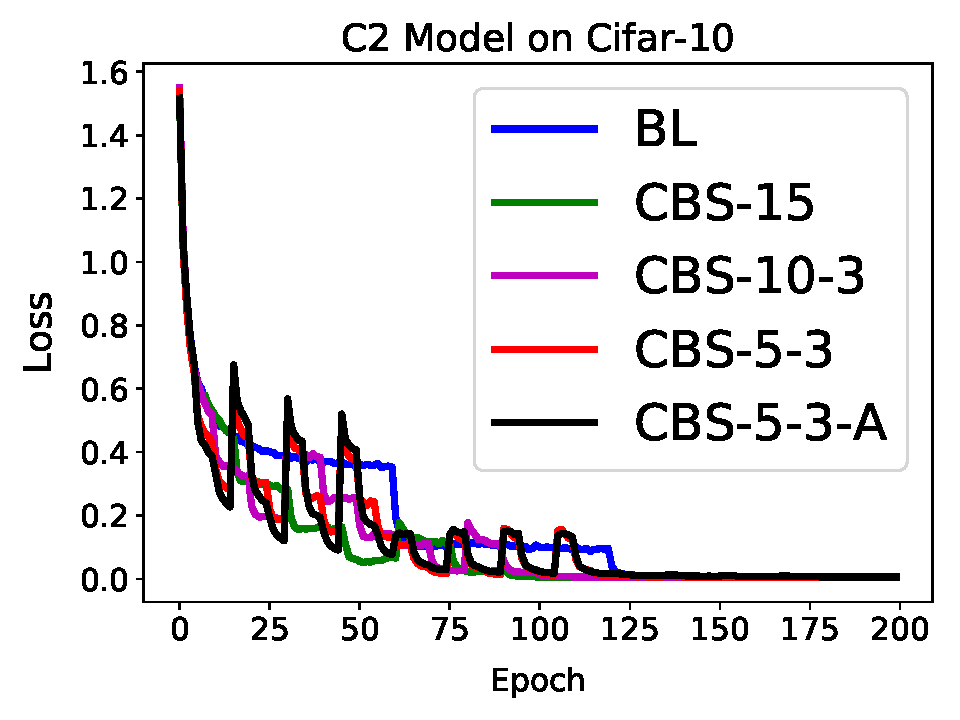
\includegraphics[width=.4\textwidth]{fig/loss_c1.pdf}
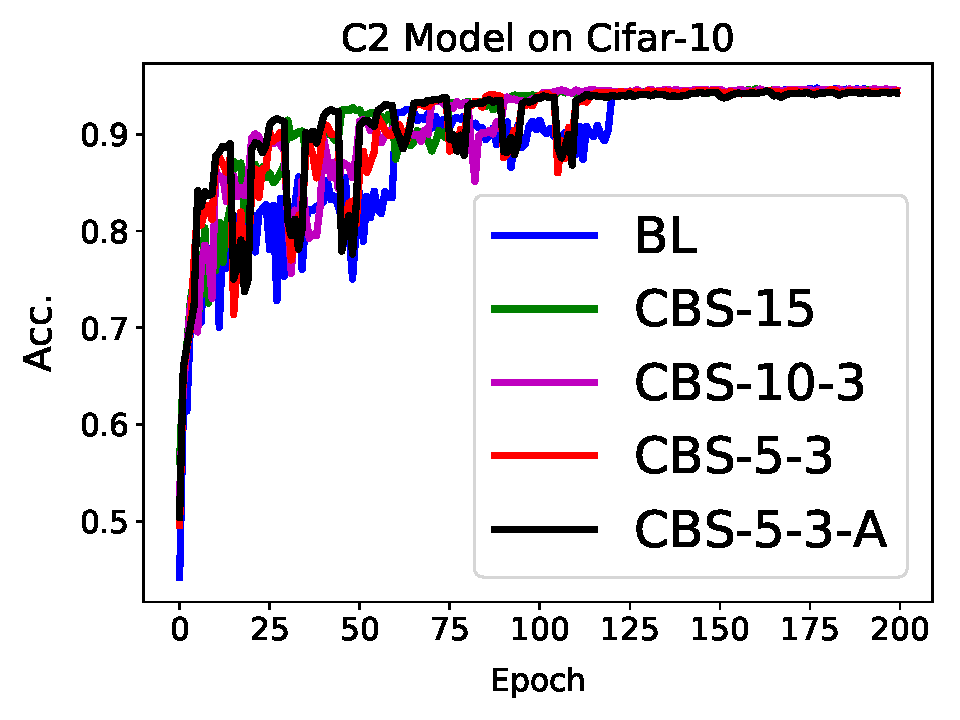
\includegraphics[width=.4\textwidth]{fig/acc_c1.pdf}
  \caption{\footnotesize C2 model (WResNet) on Cifar-10. Training set loss (left), and testing set accuracy (right), evaluated as a function of epochs}

  \label{fig:wresnet_cifar10}
\end{figure}

\begin{figure}[!htbp]
  \centering
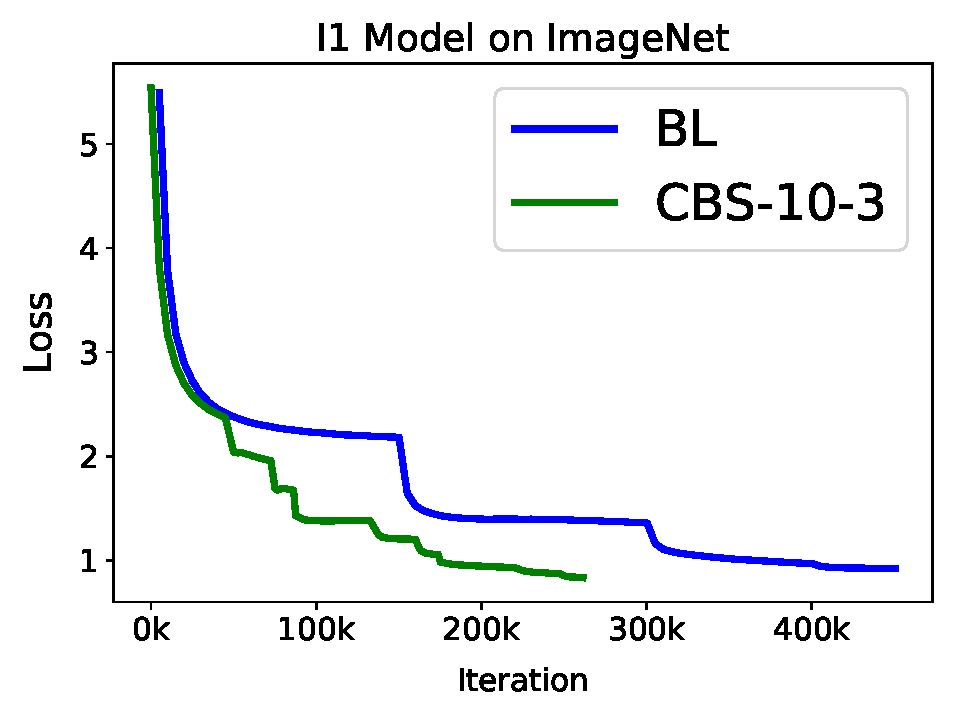
\includegraphics[width=.4\textwidth]{fig/loss_iter_I1.pdf}
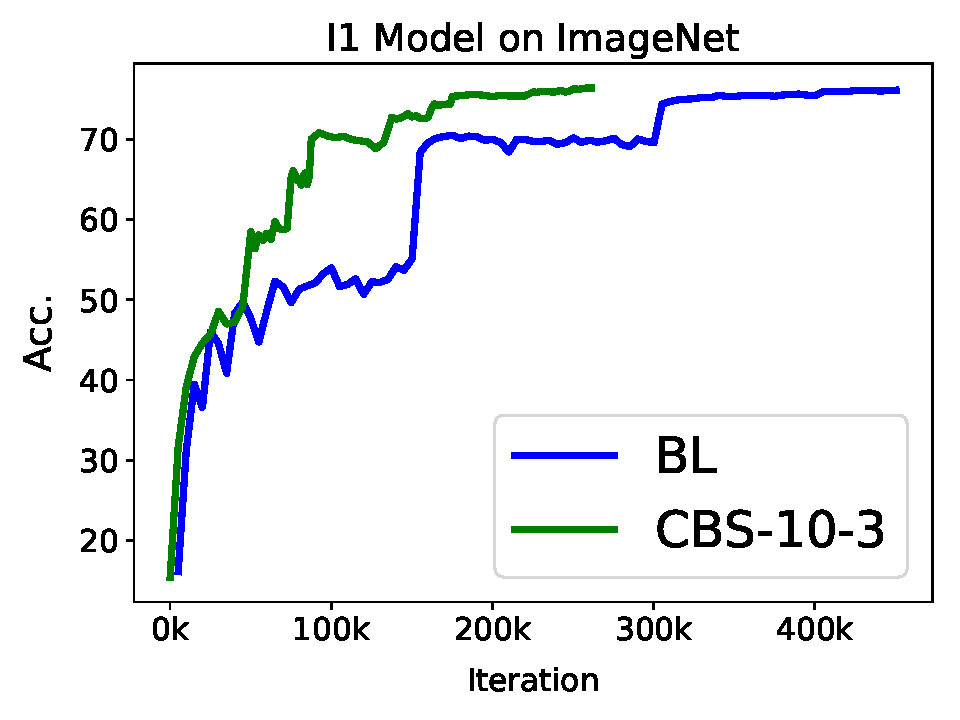
\includegraphics[width=.4\textwidth]{fig/acc_iter_I1.pdf}
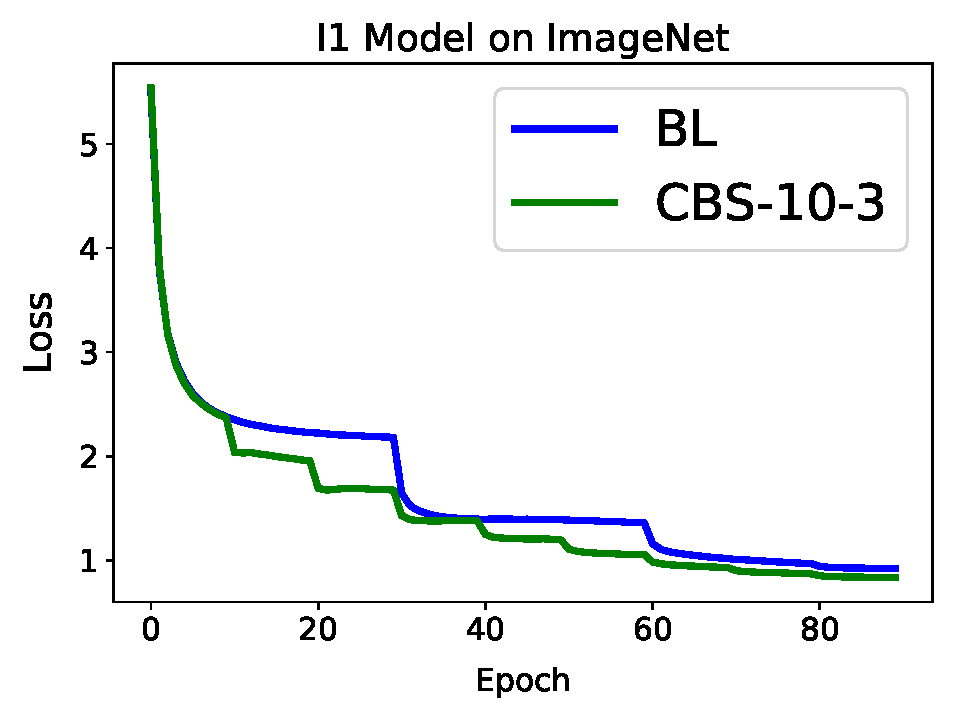
\includegraphics[width=.4\textwidth]{fig/loss_I1.pdf}
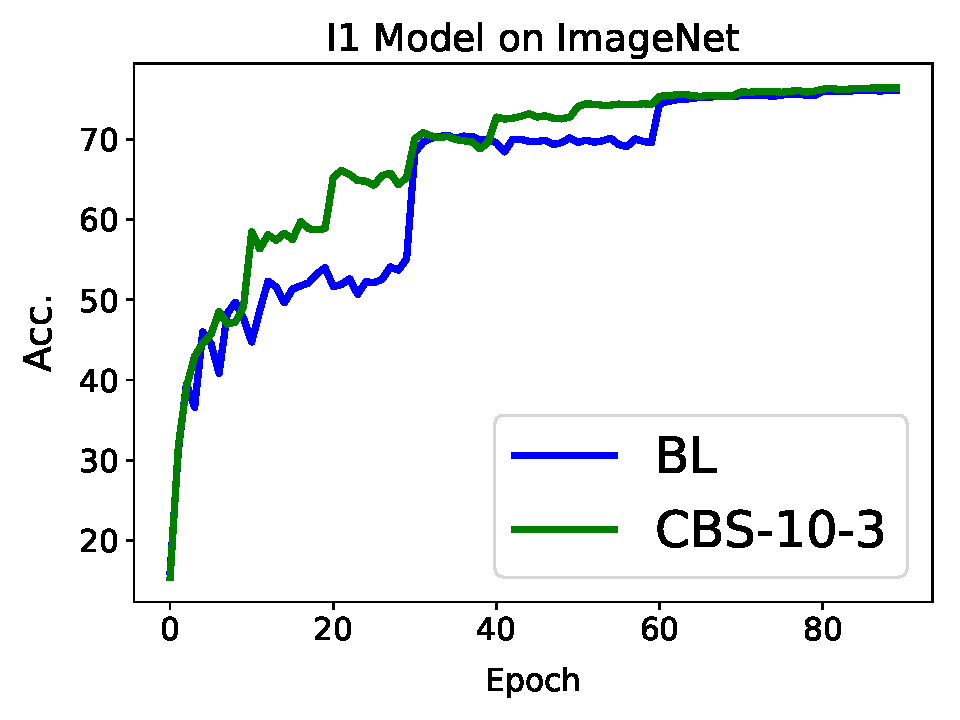
\includegraphics[width=.4\textwidth]{fig/acc_I1.pdf}

  \caption{\footnotesize I1 model (ResNet50) on ImageNet. Training set loss (left), and testing set accuracy (right), evaluated as a function of iterations (above) and epochs (below).}
  \label{fig:cbs_imagenet}
\end{figure}

\subsection{Sub-optimal Initialization}\label{sec:bad_init}
Various effective initialization methods~\cite{glorot2010understanding,he2015delving,saxe2013exact,mishkin2015all}
have been proposed previously; however, when presented with new architectures and new tasks,
initialization still needs to be explored empirically and often the final
performance varies greatly with different initializations. In this section, we test if
CBS schedules can alleviate the problem of sub-optimal initialization.

We test a Gaussian initialization with mean $0$ and standard deviation $0.1$ on 
an AlexNet-like model (C1). The baseline (BL) training follows the same setting as described in 
Appendix~\ref{sec:training_outline} and achieves final accuracy $84.27\%$. For CBS, we use cycle width of 10 with 3 steps.
In particular, CBS$_1$ denotes a constant learning rate, and achieves final accuracy $85.41\%$. CBS$_2$ decays the learning rate by a factor of 5 at
epoch 75 and achieves final accuracy $84.95\%$. 
We keep learning rate high during training because a high noise 
level helps $\theta$ escape sub-optimal local minima. 
Notice that all CBS methods achieve better generalization performance than the baseline.